\documentclass[11pt, letterpaper]{article}
\usepackage[margin=1in]{geometry}
\usepackage[utf8]{inputenc}
\usepackage[all]{xy}
\usepackage[hidelinks]{hyperref}
\usepackage{url, amsmath, amsfonts, stmaryrd, amssymb, amsthm, mathtools, enumerate, bm, geometry, tabularx, graphicx, caption}

\title{\textbf{Understanding Flight Delays}\\\textbf{CSE 519: Data Science Fundamentals}\\\textbf{Project Progress Report}}
%\author{
%  Kai Li\\
%  \texttt{kai.li@stonybrook.edu}
%  \and
%  Peng Fei Yao\\
%  \texttt{pengfei.yao@stonybrook.edu}
%}
\date{Stony Brook University --- \today}

\begin{document}
\maketitle

\section{Introduction and Objectives}
Airline flight delay has become one of the most serious issues across the world in the 21st century. This project concerns the influence of flight delays on airports and airlines using different classifications. We are also interested in predicting when flight delays are likely to occur in terms of modeling the total minutes delayed in a given time frame. The purpose of the progress report is to extend the research based on the flight delay backgrounds and analysis discussed in the project proposal. We will continue using the general definition of ”flight delay” and ”on-time” adopted by FAA, BTS, and NAS. This progress report proceeds as follows: Section \ref{sec:data} considers a detailed discussion about our comprehension of the datasets and how we used them. Extra intermediate exploratory data analysis following up the proposal is provided in Section \ref{sec:findings}. Finally, we conclude in Section \ref{sec:improvements} by highlining future tasks we will do to finish the project.

\section{Data}\label{sec:data}
In this project, we have used five datasets. The first one of the list below is our primary dataset, where we obtain most of our flight delay, airline and airport information. The rest are secondary datasets, which are supportive data to further categorize and differentiate airlines and airports in the primary dataset. We have 123,896 total observations, including 156 missing values in the number of arrival flights delayed. Among the 156 missing values, 135 of them are also missing in all other flight delay statistics, such as the number of flights delayed due to weather. In this project, we will remove the 135 null values because the observations are missing systematically. Moreover, the rest of the 21 missing values of the number of flights delayed can be computed by the simple addition of the numbers of delays due to other factors. Interestingly, we filtered out the delay factor statistics for the 21 missing values and observed that they are all 0. Hence, we solved this issue by simply imputing the 21 missing number of flights delayed by 0.

\begin{description}
  \item[Airline On-Time Arrival Performance Data] \hfill \\ Our major dataset contains core information to report the on-time arrival performance of flights comprehensively. The dataset comes from the BTS Airline On-Time Statistics and Delay Causes \cite{web:bts1}. There are 21 features covering the airline arrival statistics from January 2012 to December 2019. For instance, the number of flights arriving at the airport, flights delayed, canceled flights, and the length of time due to various delay reasons are provided. We also added two extra variables, denoting the number of flights that arrived on-time and the delayed rate, for the sake of comparison and analysis procedures. The number of on-time arrival flights is calculated by subtracting the number of delayed, canceled, and diverted flights from the total number of arrival flights. The delayed rate is computed by the ratio of the number of delayed flights and the total number of flights arrived for each observation.
  \item[Airport Busyness Data] \hfill \\ The Airport Busyness Data is an auxiliary dataset pre-processed from the BTS Airline On-Time Statistics and Delay Causes dataset \cite{web:bts1}. After cleaning the missing values in the primary dataset, as discussed previously, we have 375 airports in the file. The 30 major airports, classified in the BTS database, will be regarded as the busiest airports. The rest of the airports are coded as less busy airports to facilitate our research.
  \item[Airline Carrier Group Data] \hfill \\ The Airline Carrier Group Data is a pre-processed secondary dataset from the BTS Aviation Support Tables database \cite{web:bts2}. BTS categorizes the airlines into 9 categories, based on the airline's carrier type and market size. The 23 airline carriers in the main dataset fall into either one of the two categories.
  \begin{description}
  \item[National Carriers] Carriers with annual revenue over \$100 million to \$1 billion
  \item[Major Carriers] Carriers with annual revenue over \$1 billion
  \end{description}
  \item[Airline Market Carrier Data] \hfill \\ Another classification to the airline companies is based on the Codeshare Agreement, presented in the BTS Air Carrier Statistics \cite{web:bts3}. Codesharing is a commercial agreement between airline companies that permits a marketing airline to put its two-letter identification code on the flights of another operating airline as they appear in CRS \cite{web:gsa}. Here, the dataset considers two divisions given the airlines' Codeshare Agreements with others.
  \begin{description}
  \item[Marketing Carriers] Carriers have their own market flights and regional codeshare partners
  \item[Regular Carriers] The rest of the carriers not belonging to the category Marketing Carriers
  \end{description}
  \item[Airline Carrier History Data] \hfill \\ Last but not least, the Airline Carrier History Data provides detailed information on the time of the establishment of all airlines from the BTS Air Carrier Statistics \cite{web:bts3}. In particular, the dataset separates the history for airlines that had a changed code/name previously for our analysis. After a careful data cleaning, we can regard the establishment and ending (a null value indicates that the airline is still in operation) years as continuous variables for further analysis.
\end{description}

\section{Current Findings}\label{sec:findings}
\subsection{Delays in Busiest Airports and the others}
In the proposal, we introduced that the average annual delay rates are about 2 to 3 percent higher for the busiest airports from 2012 to 2019, except for 2014. Here, we present another useful bar plot, shown in Figure \ref{fig:bar_plot}, to see if there are seasonal effects on the flight delay performance by month. We noted that the monthly delay rates for busiest airports are about 1 to 2 percent higher than less busy airports for each month. Besides that, the monthly delay rates, in general, are much higher during June, July, and August compared to September, October, and November for all airports. This may suggest particular seasonal patterns behind.

\begin{figure}[h!]
\centering
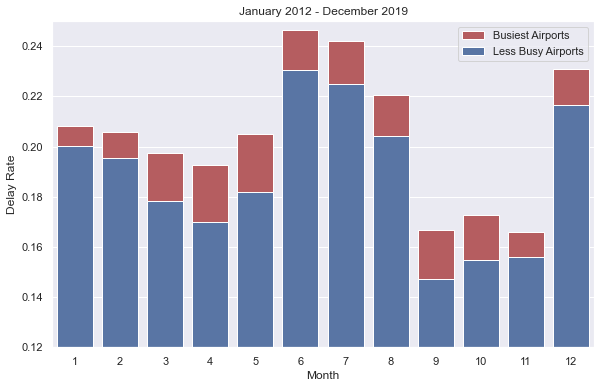
\includegraphics[width = 0.75\textwidth]{bar_plot}
\caption{Flight Delay Rate for Buiest Airports and Less Busy Airports by Month}\label{fig:bar_plot}
\end{figure}

\subsection{Delays Versus Airline Market Size}
We showed in our proposal that smaller airline companies may have a higher probability of flight delay compared to larger airline carriers through an exploratory data analysis on yearly delay rates for both carriers. Similarly, we want to further investigate the relationship in terms of monthly delay rate to see if the conclusion holds. Table \ref{tab:carrier} shows a very similar conclusion that national carriers have about 1\% to 2\% more delay rates per month than major carriers.
 
\begin{table}[h!]
\centering
\resizebox{\linewidth}{!}{
\begin{tabular}{lcccccccccccc}
  & 1 & 2 & 3 & 4 & 5 & 6 & 7 & 8 & 9 & 10 & 11 & 12 \\ 
\hline
 National & 21.37 & 21.44 & 19.32 & 18.88 & 19.92 & 24.69 & 23.98 & 21.89 & 16.33 & 17.50 & 17.24 & 22.80 \\  
 Major & 19.62 & 19.00 & 17.81 & 16.89 & 18.16 & 22.79 & 22.36 & 20.25 & 14.62 & 15.11 & 15.13 & 21.58 \\
\end{tabular}}\caption{Delay Rate (in Percentage) for National Carriers and Major Carriers}\label{tab:carrier}
\end{table}

Besides classifying airlines into their annual revenues, we also categorized them based on whether they have their market flights and regional codeshare partners. If they do, they are regarded as marketing carriers in this project. Otherwise, they are considered regular carriers. From Table \ref{tab:market}, there is no monotone formula of the monthly flight delay rates based on our analysis. In particular, during the second and the third quarters, marketing carriers appear to have a 1\% to 2\% more delay rates than regular carriers, while the first and the last quarters exhibit an opposite observation. We conjecture that a more sophisticated relationship, such as quadratic and cubic, exists between marketing carriers and delay.

\begin{table}[h!]
\centering
\resizebox{\linewidth}{!}{
\begin{tabular}{lcccccccccccc}
  & 1 & 2 & 3 & 4 & 5 & 6 & 7 & 8 & 9 & 10 & 11 & 12 \\ 
\hline
 Marketing & 19.04 & 18.75 & 18.38 & 17.68 & 19.41 & 24.10 & 23.73 & 21.27 & 15.18 & 15.36 & 15.31 & 21.23 \\  
 Regular & 21.46 & 20.93 & 18.23 & 17.40 & 18.00 & 22.67 & 21.94 & 20.26 & 15.17 & 16.51 & 16.41 & 22.82 \\
\end{tabular}}\caption{Delay Rate (in Percentage) for Marketing Carriers and Regular Carriers}\label{tab:market}
\end{table}

\subsection{Delays Versus Airline Establishment Time}
We are interested in whether airline companies that were established earlier have a lower delay rate from January 2012 to December 2019. The following Figure \ref{fig:reg_plot} is a scatter plot with a regression line demonstrating the relationship between delay rates and years of establishment. We considered the operating airlines with ending years of 2021 to measure the linear association. Note that the slope of the regression line is about 0, which depicts that possibly the years of establishment do not significantly affect the flight delay rate.

\begin{figure}[h!]
\centering
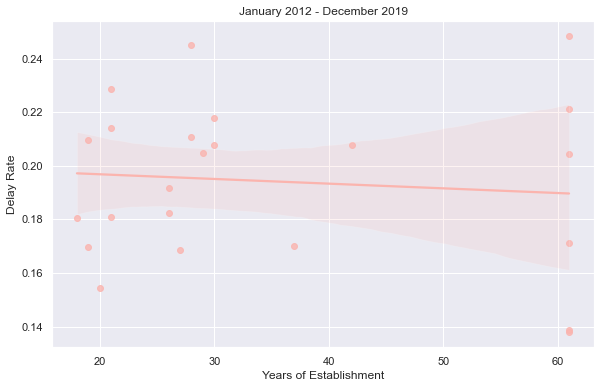
\includegraphics[width = 0.75\textwidth]{reg_plot}
\caption{Flight Delay Rate for Years of Establishment}\label{fig:reg_plot}
\end{figure}

\subsection{Modeling and Prediction}
To build a satisfactory prediction model, we started with building an elementary baseline model. The baseline model is based on a first-order multiple linear regression model due to its fast-learning characteristics and simplicity in terms of implementation and results interpretation. In Python, we used the \texttt{sklearn.linear\_model.LinearRegression} function to reach our goal. Furthermore, we built a simple baseline model with obviously correlated features. In particular, we selected variables month, an airport busy or not, and carrier group as the regressors with the total minutes of delay as the response. We will then compare our sophisticated model to the baseline model to measure improvement. Last but not least, we used the default hyperparameters in the function to train the model. That is, the baseline model will have an intercept with unnormalized regressors.

To properly evaluate the baseline model performance, we split the entire dataset into a training and a validation set, which are 80\% and 20\% of the original data, respectively, chosen at random. The training set was used to build the multiple linear regression model, with several performance metrics, selected based on our discretion, to score the predictions on the validation set.

The baseline model has a coefficient of determination of 13.89\%, an adjusted coefficient of determination of 13.88\%, and a mean squared logarithmic error of 4.18. We believe the baseline model provides ample insights to further increase the model performance, as discussed in Section \ref{sec:improvements}.

\section{Future Improvements}\label{sec:improvements}
\begin{description}
  \item[Feature Selection] \hfill \\ We selected our features based on the initial judgment of the relationship among the variables in the baseline model. Next we analyze the graphical exploratory data analysis results from the previous findings in Section \ref{sec:findings}.
  \item[Feature Engineering] \hfill \\ Feature engineering is critically important in improving the prediction model performance. We will try various feature engineering techniques such as feature creation and transformation to see if these features provide a better machine learning outcome.
  \item[Hyperparameter Tuning] \hfill \\ Hyperparameter tuning is a process of building the optimal model among all possible models with different hyperparameters. A grid search or a randomized search can be very helpful in testing different hyperparameters and output performance with a suitable scoring metric. Validation curves can help observe overfitting or underfitting for different hyperparameter values. Especially, the training scores and the validation scores for different combinations of hyperparameters can be used for hyperparameter tuning.
  \item[Cross-validation] \hfill \\ Cross-validation helps to obtain more generalized relationships among the features. In particular, we prefer a $k$-fold cross-validation technique to proceed with the predictive modeling.
  \item[Error and Score Metric] \hfill \\ Choosing the best error and score evaluation metric releases useful information to explain the goodness of fit. The ideal metric to optimize is model-specific and require extra analysis.
  \item[Testing Multiple Models/Algorithms] \hfill \\ Discovering additional models provides valuable recommendations for the best performance model. Both simple and more complicated models will be tried. For example, we are interested in building time-series regression, lasso/ridge regression, random forest, and neural network machine learning models for comparison.

\end{description}

\bibliographystyle{abbrv}
\bibliography{refs}

\end{document}